\chapter{Dictionaries for Special Keys}

\tikzset{
  tri/.style={circle,draw,fill=blue!6,minimum size=3.5mm,inner sep=0pt},
  tlf/.style={draw,rounded corners,fill=green!10,font=\scriptsize\ttfamily,inner sep=2pt},
  el/.style={font=\scriptsize\ttfamily,inner sep=1pt}
}

The comparison lower bound applies to searching too: any comparison-based search
in a set of $n$ keys needs $\Omega(\log n)$ comparisons (a decision tree must
have $n + 1$ distinguishable outcomes). To do better we must exploit the
structure of the keys: numbers (interpolation search) or strings (tries).

\section{Lower Bound for Search}

\begin{theorem}
In the comparison model, \code{search} requires $\Omega(\log n)$ comparisons in
the worst case.
\end{theorem}
\begin{proof}
A decision tree for search must have at least $n + 1$ leaves (one for each
key found, plus ``not found''). A binary tree with $n + 1$ leaves has height at
least $\log(n+1)$.
\end{proof}

\section{Interpolation Search}

Binary search on a sorted array always probes the middle. If keys are numbers
spread roughly uniformly, we can guess where $k$ should be, like looking up a
name in a phone book.

\begin{lstlisting}
interpolation-search(A[0..n-1], k):
  l <- 0; r <- n - 1
  while l <= r and A[l] <= k <= A[r] do
    if A[l] = A[r] then
      if A[l] = k then return l else return "not found"
    m <- l + floor( (k - A[l]) / (A[r] - A[l]) * (r - l) )
    if A[m] = k then return m
    else if A[m] < k then l <- m + 1
    else r <- m - 1
  return "not found"
\end{lstlisting}

Binary search uses $m = l + \floor{\frac12 (r - l)}$; interpolation search
replaces $\frac12$ by the fraction $\frac{k - A[l]}{A[r] - A[l]}$.
Geometrically, it draws the line through $(l, A[l])$ and $(r, A[r])$ and probes
where that line reaches height $k$:

\begin{center}
\begin{tikzpicture}[x=0.75cm,y=0.05cm]
  \draw[-{Stealth}] (0,0) -- (10,0) node[right,font=\scriptsize]{index};
  \draw[-{Stealth}] (0,0) -- (0,105) node[above,font=\scriptsize]{key};
  \foreach \i/\v in {0/2,1/9,2/21,3/30,4/38,5/52,6/58,7/71,8/80,9/94} \fill[blue!60!black] (\i,\v) circle (1.8pt);
  \draw[thick,orange!80!black] (0,2) -- (9,94);
  \draw[densely dashed] (0,62) node[left,font=\scriptsize]{$k$} -- (5.86,62) -- (5.86,0) node[below,font=\scriptsize]{$m$};
  \node[font=\scriptsize,anchor=west] at (0.15,6) {$A[l]$};
  \node[font=\scriptsize,anchor=east] at (8.9,98) {$A[r]$};
\end{tikzpicture}
\end{center}

\begin{example}
$A = [0, 10, 20, 30, 40, 50, 60, 70, 80, 90]$, search 70:
$m = 0 + \floor{\frac{70}{90}\cdot 9} = 7$. Found in one probe.
\end{example}

\paragraph{Analysis.}
\begin{itemize}
  \item If keys are uniformly distributed, the expected time satisfies
        $T(n) = T(\sqrt n) + \Theta(1)$, giving $\Theta(\log \log n)$. (Intuition:
        after one probe the expected distance to the target is about $\sqrt n$.)
  \item Worst case $\Theta(n)$: e.g.\ $A = [1, 2, \ldots, n-1, 10^{100}]$, search
        $n - 1$: each probe moves $l$ by one.
\end{itemize}

\begin{aside}
A variant that combines interpolation with a fallback to binary steps (or
galloping) avoids the linear worst case while keeping good average behaviour.
\end{aside}

\section{Tries}

Now keys are strings over an alphabet $\Sigma$ (often $\Sigma = \{0,1\}$). Comparing
two strings costs time proportional to their common prefix, so a balanced BST of
strings of length $m$ costs $\bigO(m\log n)$ per search. Tries get $\bigO(m)$.

\begin{definition}
A \emph{trie} (from re\emph{trie}val; also \emph{radix tree} or \emph{digital
search tree}) is a tree in which each edge is labelled with a character, and
the path from the root to a node spells a prefix. Each key is stored at the
node reached by its characters.
\end{definition}

\begin{remark}
To ensure no key is a prefix of another (which would put a key at an internal
node), append an end-of-word symbol \$ to every key. Then all keys are stored
at leaves. Alternatively, mark internal nodes with a flag ``a word ends here''.
\end{remark}

\begin{example}
Binary trie for $\{00\$, 0001\$, 01001\$, 011\$, 0110\$, 110\$, 1101\$, 111\$\}$:
from the root, branch on bit 0, bit 1, \ldots, with each \$ edge ending at a leaf.
\begin{center}
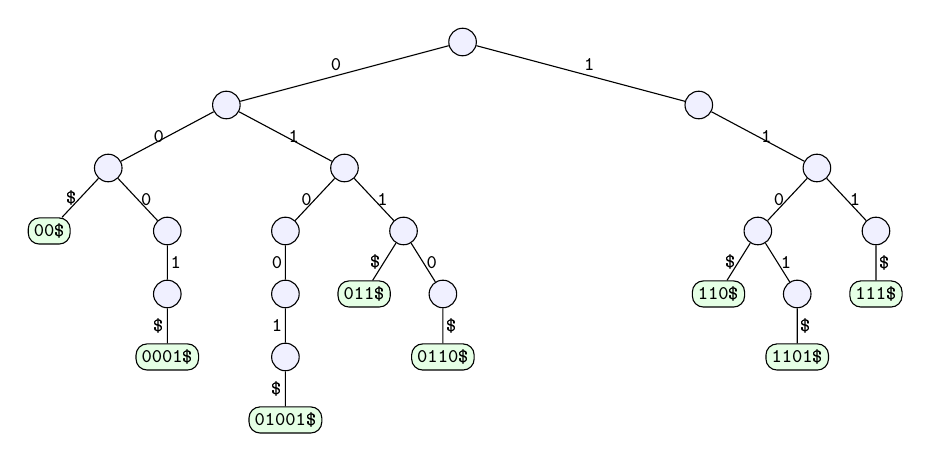
\begin{tikzpicture}[level distance=8mm,
  level 1/.style={sibling distance=60mm},
  level 2/.style={sibling distance=30mm},
  level 3/.style={sibling distance=15mm},
  level 4/.style={sibling distance=10mm},
  level 5/.style={sibling distance=10mm},
  level 6/.style={sibling distance=10mm},
  edge from parent/.style={draw}]
  \node[tri] {}
    child {node[tri] {}
      child {node[tri] {}
        child {node[tlf] {00\$} edge from parent node[el,left] {\$}}
        child {node[tri] {}
          child {node[tri] {} child {node[tlf] {0001\$} edge from parent node[el,left] {\$}} edge from parent node[el,right] {1}}
          edge from parent node[el,right] {0}}
        edge from parent node[el,left] {0}}
      child {node[tri] {}
        child {node[tri] {}
          child {node[tri] {} child {node[tri] {} child {node[tlf] {01001\$} edge from parent node[el,left] {\$}} edge from parent node[el,left] {1}} edge from parent node[el,left] {0}}
          edge from parent node[el,left] {0}}
        child {node[tri] {}
          child {node[tlf] {011\$} edge from parent node[el,left] {\$}}
          child {node[tri] {} child {node[tlf] {0110\$} edge from parent node[el,right] {\$}} edge from parent node[el,right] {0}}
          edge from parent node[el,right] {1}}
        edge from parent node[el,right] {1}}
      edge from parent node[el,above left] {0}}
    child {node[tri] {}
      child[missing]
      child {node[tri] {}
        child {node[tri] {}
          child {node[tlf] {110\$} edge from parent node[el,left] {\$}}
          child {node[tri] {} child {node[tlf] {1101\$} edge from parent node[el,right] {\$}} edge from parent node[el,right] {1}}
          edge from parent node[el,left] {0}}
        child {node[tri] {} child {node[tlf] {111\$} edge from parent node[el,right] {\$}} edge from parent node[el,right] {1}}
        edge from parent node[el,right] {1}}
      edge from parent node[el,above right] {1}};
\end{tikzpicture}
\end{center}

\end{example}

\subsection{Operations}

\begin{lstlisting}
trie-search(v, x, d):     // v node, x key, d = current depth
  if v is a leaf then return v
  c <- x[d]  (or $ if d = |x|)
  if v has a child w on edge c then
    return trie-search(w, x, d+1)
  else return "not found"
\end{lstlisting}

\begin{itemize}
  \item \code{search(x)}: follow the characters of $x$; fail if a child is missing.
  \item \code{insert(x)}: search; when a child is missing, create new nodes for
        the remaining characters (ending with a leaf for \$).
  \item \code{delete(x)}: search to the leaf, delete it, then delete ancestors
        that now have no children.
\end{itemize}
All run in $\Theta(|x|)$ time, independent of $n$. Other useful operations:
prefix search (all keys starting with $p$), successor/predecessor, and sorting
(a pre-order traversal outputs keys in lexicographic order).

\section{Variations of Tries}

\subsection{No leaf labels}
Keys need not be stored at leaves, since the path spells them; saves space.

\subsection{Pruned tries}
Stop adding nodes once the key is unique: a node has a child only if it has at
least two descendants. The leaf stores the full key, and search must compare
$x$ with the stored key at the end. This is the trie implicit in MSD radix sort.

\subsection{Compressed Tries (Patricia Tries)}

\begin{definition}
A \emph{compressed trie} (Patricia: Practical Algorithm To Retrieve Information
Coded In Alphanumeric) removes all internal nodes with only one child. Each
internal node stores the \emph{index} of the character to test next; each leaf
stores the full key.
\end{definition}

Since every internal node has at least two children, a compressed trie with $n$
keys has at most $n - 1$ internal nodes: $\Theta(n)$ space regardless of key
lengths.

\begin{lstlisting}
patricia-search(v, x):
  if v is a leaf then
    if x = v.key then return v else return "not found"
  d <- v.index                 // character position to test
  c <- x[d]  (or $ if d = |x|; "not found" if d > |x|)
  if v has a child w on edge c then return patricia-search(w, x)
  else return "not found"
\end{lstlisting}
Note the final comparison with the stored key is required, since skipped
positions were never checked.
\begin{center}
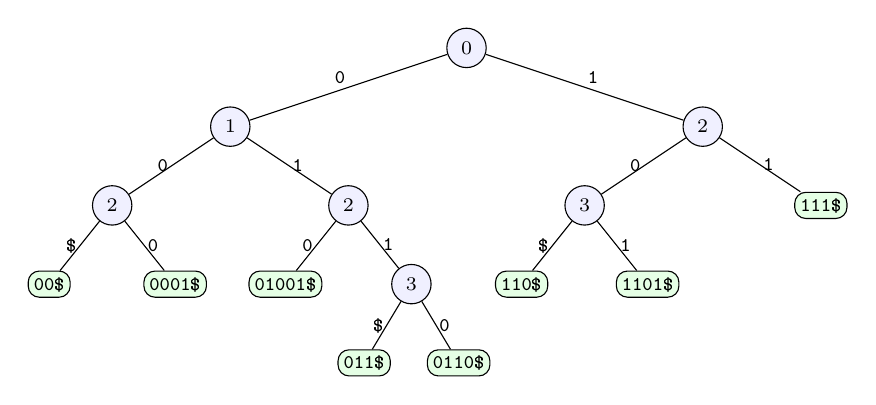
\begin{tikzpicture}[level distance=10mm,
  level 1/.style={sibling distance=60mm},
  level 2/.style={sibling distance=30mm},
  level 3/.style={sibling distance=16mm},
  level 4/.style={sibling distance=12mm},
  ix/.style={circle,draw,fill=blue!6,minimum size=5mm,inner sep=0pt,font=\scriptsize}]
  \node[ix] {0}
    child {node[ix] {1}
      child {node[ix] {2}
        child {node[tlf] {00\$} edge from parent node[el,left] {\$}}
        child {node[tlf] {0001\$} edge from parent node[el,right] {0}}
        edge from parent node[el,left] {0}}
      child {node[ix] {2}
        child {node[tlf] {01001\$} edge from parent node[el,left] {0}}
        child {node[ix] {3}
          child {node[tlf] {011\$} edge from parent node[el,left] {\$}}
          child {node[tlf] {0110\$} edge from parent node[el,right] {0}}
          edge from parent node[el,right] {1}}
        edge from parent node[el,right] {1}}
      edge from parent node[el,above left] {0}}
    child {node[ix] {2}
      child {node[ix] {3}
        child {node[tlf] {110\$} edge from parent node[el,left] {\$}}
        child {node[tlf] {1101\$} edge from parent node[el,right] {1}}
        edge from parent node[el,left] {0}}
      child {node[tlf] {111\$} edge from parent node[el,right] {1}}
      edge from parent node[el,above right] {1}};
\end{tikzpicture}
\end{center}
The compressed trie for the same keys as the binary trie above: each internal
node shows the (0-based) index of the bit it tests, and only 7 internal nodes
remain for 8 keys.


\paragraph{Insert.} Search for $x$; this leads to some leaf (or fails at a node).
Compare $x$ with any key $y$ in that subtree to find the first index $d$ where
they differ. Walk back up to where $d$ belongs (between a parent with smaller
index and a child with larger index), and create a new internal node with index
$d$ there, with two children: the old subtree and a new leaf for $x$.

\paragraph{Delete.} Remove the leaf; if its parent now has only one child,
remove the parent and connect the sibling to the grandparent.

All operations take $\bigO(|x|)$ time.

\subsection{Multiway Tries}

For a larger alphabet (e.g.\ $|\Sigma| = 26$ letters plus \$), each node has up to
$|\Sigma| + 1$ children. How to store the children?
\begin{center}
\begin{tabular}{lll}
\toprule
Child storage & Time per node & Space per node\\
\midrule
Array of size $|\Sigma|+1$ & $\bigO(1)$ & $\Theta(|\Sigma|)$\\
List of children & $\bigO(|\Sigma|)$ & $\Theta(\#\text{children})$\\
Balanced BST / AVL of children & $\bigO(\log|\Sigma|)$ & $\Theta(\#\text{children})$\\
Hash table of children & $\bigO(1)$ expected & $\Theta(\#\text{children})$\\
\bottomrule
\end{tabular}
\end{center}
In practice an array is fastest for small $\Sigma$ and a hash map otherwise.
Multiway tries can also be compressed.

\section{Summary}
\begin{center}
\begin{tabular}{lll}
\toprule
Structure & Search time & Space\\
\midrule
Binary search (sorted array) & $\Theta(\log n)$ & $\Theta(n)$\\
Interpolation search & $\Theta(\log\log n)$ avg, $\Theta(n)$ worst & $\Theta(n)$\\
Trie (strings, length $m$) & $\Theta(m)$ & $\bigO(\text{total length})$\\
Compressed trie & $\Theta(m)$ & $\Theta(n)$ nodes\\
\bottomrule
\end{tabular}
\end{center}
\begin{itemize}
  \item Comparison-based search needs $\Omega(\log n)$; special keys let us beat it.
  \item Interpolation search guesses the position from key values.
  \item Tries store strings by their characters; compressed tries skip unary
        nodes and test only the positions that distinguish keys, but must verify
        the full key at the leaf.
\end{itemize}
